\newpage
\section{R!-Relevante Dinge}
\subsection{Befehle}
\label{subsec:RBefehler}
\begin{tabularx}{\linewidth}{p{0.15\linewidth} X X}
	\textbf{Funktion}	&	\textbf{Befehl} 							&\textbf{Kommentar}\\\hline
	Plot erstellen		& \textit{plot(YAchse$\sim$XAchse,data=VarName)}&Namen der Y- und X-Achse müssen Spaltennamen in der Variabel
																		 sein\\\hline
	Lineare Regression	&\textit{lm(YAchse$\sim$XAchse,data=VarName)}	&Liefert Koeffizienten für lin. Regression der Y-Achse auf
																		X-Achse. \newline
																		Intercept = $\alpha$\newline
																		VarNameX  = $\beta$ der betroffenen Variabel\newline
																		Ouput von summary eines linearen eines Parameter \ref{subsubsec:summary} \\
						&\textit{lm(YAchse$\sim$X1Achse+X2Achse,data=VarName)}	
																		&Multiple lineare Regression, möglich mit beliebige vielen \textit{XnAchsen}, Summary-Output von einem Modell für multiple lineare Regression: Kapitel \ref{subsubsec:MultipleLineareRegressionR}\\\hline
	Zusammenfassung		&\textit{summary(varname)}						&Liefert die Zusammenfassung eines Elements, varname kann 
																		z.B. in von lm-Erhaltene Var sein, siehe \ref{subsubsec:summary}\\\hline
	Lin. Koeffizienten eintragen&\textit{abline(varName)}				&Zeichnet die Lin. Regression in eine Grafik, varName vom
																		 Typ \textit{lm}\\\hline
	Eine Spalte ansprechen&\textit{varName\$SpaltenName}				&Spricht eine Spalte der Variabel an, kann auch gebraucht
																		 werden um eine Spalte hinzuzufügen
																		 z.b. \textit{A\$x$<-$1/A\$B} spalte x $=\frac{1}{B}$\\\hline 
	Konfidenzintervall	&\textit{confint(lm-objekt, $\left[\text{\textit{parm=2}}\right]$,level=confLvl)}
																		&Konfidenzintervall, damit Konfidenzlevel\% der Werte 
																		innerhalb dieses
																		Bereiches ist. Bei mehreren Parameter kann optional der gewünschte Parameter angegeben werden, wenn nichts angegeben gibt Wert für alle Parameter. Somit liegt für z.B. 99\% $\rightarrow$ und parameter 2 (Steigung): Steigung muss zwischen den zwei Ausgegebenen Werten für 0.5\% und 99.5\% liegen, um ein Konfidenzintervall von 99\% zu erreichen.\\\hline
	Vertrauens- und Prognoseintervall &sieh Kapitel \ref{subsubsec:VertrauensUndPrognoseintervall}&Entsprechen Kapitel
																		 \ref{subsubsec:VertrauensUndPrognoseBereich}\\\hline
	Eine Eintrage weglassen&\textit{myData$\left[\right.$-19,$\left.\right]$}& Lässt den Datenpunkt 19 Weg\\
						&\textit{...(YAchse$\sim$XAchsee,data=myVar, subset=-19)}&Lässt überall den Eintrag 19 Weg\\\hline
	Anova-Test			&aov(YAchse$\sim$X1Achse+X2Achse,data=myData)	&F-Statistik für die zwei Beobachtungen X1 und X2\\
						&aov(YAchse$\sim$X1Achse$\ast$X2Achse,date=myData)&F-Statistik für die zwei Beobachtungen X1 und X2, inkl. 
																		der. Relevanz deren Wechselwirkung. Wechselwirkung in Output dargestellt als X1:X2. Wenn p-Wert $>0.05$ kann $H_0$ \underline{nicht} verworfen werden, d.h. Es kann sein, dass diese Wechselwirkung \underline{keinen} Einfluss hat.\\\hline
	Daten eingeben		&\textit{data.frame(...)}						&Siehe Kapitel \ref{subsubsec:Dataframe}\\\hline
\end{tabularx}

\clearpage
\subsection{Deutung des R!-Outputs}
\subsubsection{Summary}
Achtung: Ggf. ist das mit dem T-Wert nicht korrekt! Falls nötig und Zeit noch prüfen!
\label{subsubsec:summary}
\begin{figure}[h!]
	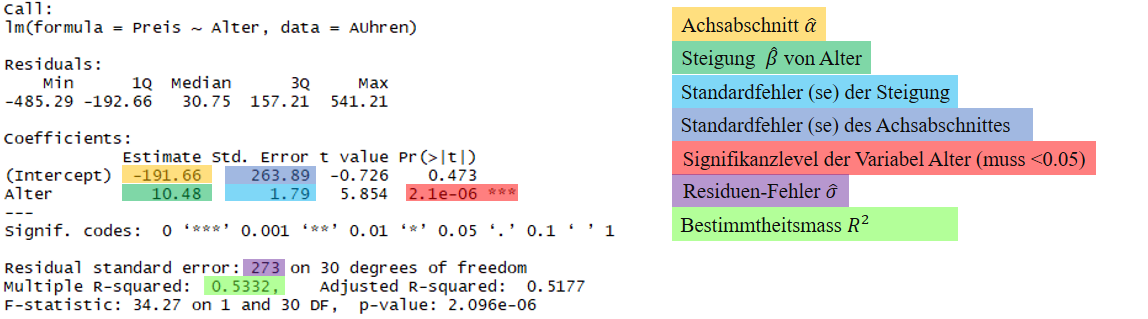
\includegraphics[width=0.9\linewidth]{figures/RSummary}
\end{figure}

\subsubsection{Vertrauens- und Prognoseintervall}
\label{subsubsec:VertrauensUndPrognoseintervall}
\begin{figure}[!h]
	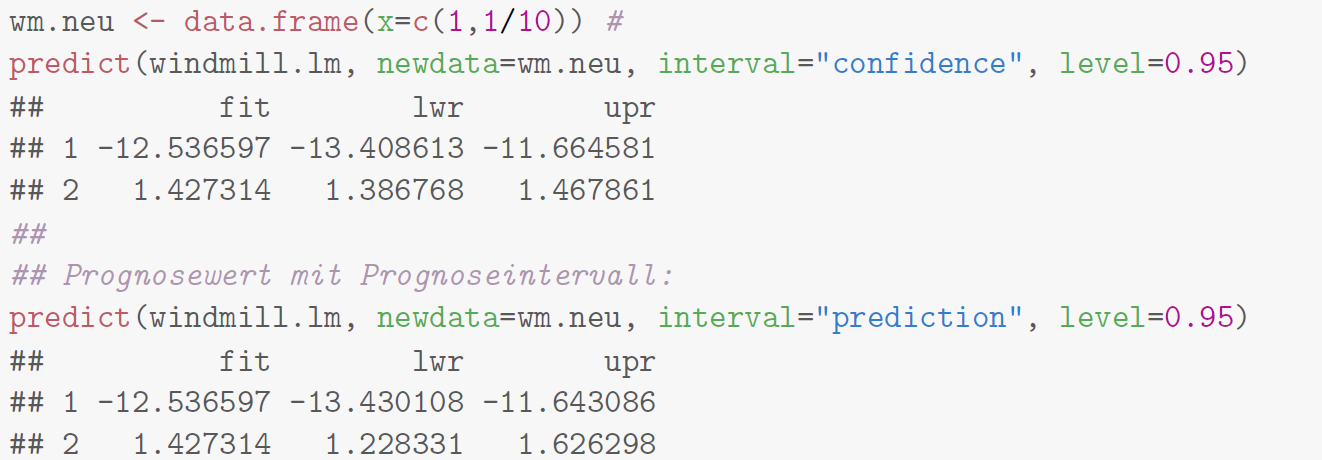
\includegraphics[width=0.5\linewidth]{./figures/Rprediction}
	\caption{\textit{Quelle:} \cite{C:Prediction}}
	\label{fig:rprediction}
\end{figure}

\begin{itemize}
	\item [1.]\textit{data.frame(x=c(1,1/10)} erstellt Vektor x mit 1 und 0.1 ($\rightarrow$ Werte für $x_0$ )
	\item [2.]\textit{$\left[\ldots\right]$interval="confidence", level=0.95$\left.\right)$} Konfidenzintervall (Vertrauensintervall) für 95\%
	\item [3.]Obere Zeile für ersten Eintrag des Vektors (1) und untere Zeile für 2. Eintrag des Vektors
	\begin{itemize}
		\item fit = Erwartungswert, anschliessend untere und obere Grenze
		\item siehe Abbildung \ref{fig:ProgrnoseUndVertrauen} für Bedeutung der Punkte
	\end{itemize}
	\item [4.]\textit{$\left[\ldots\right]$interval="prediction", level=0.95$\left.\right)$} Konfidenzintervall für 95\%
	\begin{itemize}
		\item Liefert Prognosegrenze
	\end{itemize}
\end{itemize}

\subsubsection{Multiple Lineare Regression}
\label{subsubsec:MultipleLineareRegressionR}
\begin{figure}[!h]
	\centering
	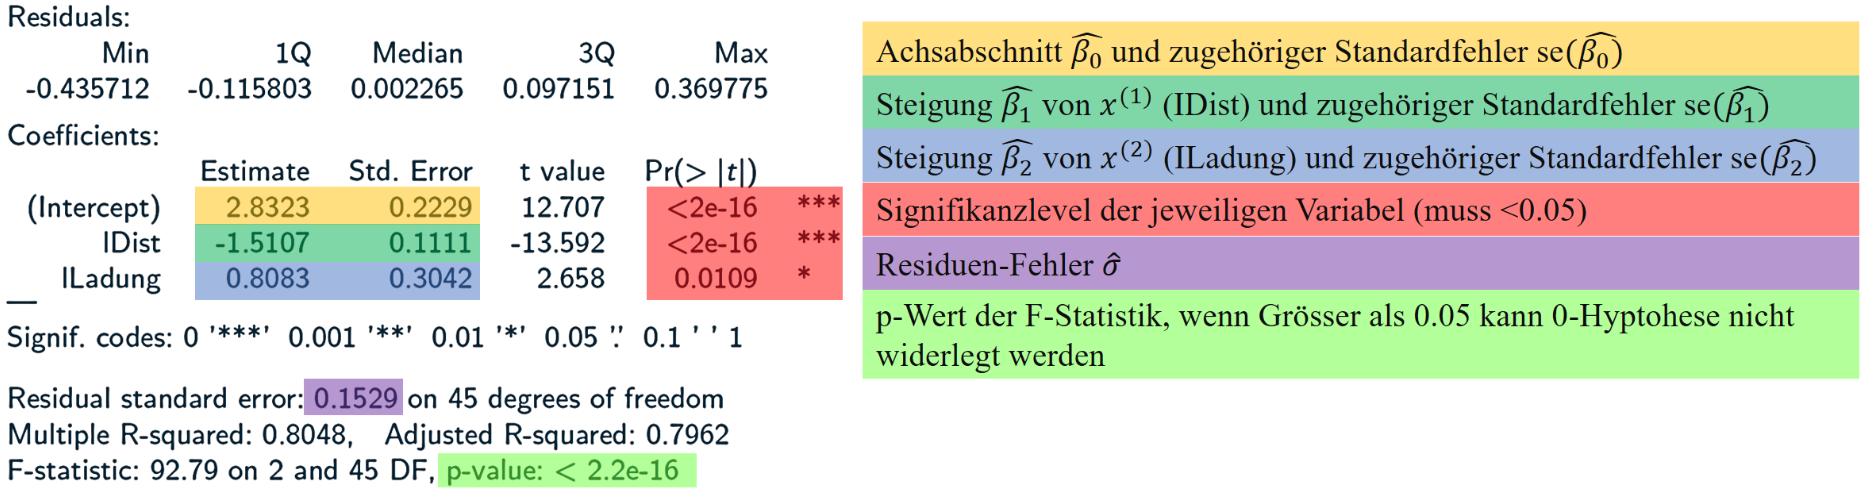
\includegraphics[width=1\linewidth]{figures/MultiReg1}
	\caption{R-Output der Multiplen Regression}
	\label{fig:multireg1}
\end{figure}


\subsubsection{Konfidenzintervall}
\label{subsubsec:konfidenzintervallR}
\begin{itemize}
	\item 95\% Intervall für jeden der Parameter
	\begin{itemize}
		\item Somit Werte mögliche Werte der Variablen damit zwischen 2.5\% und 97.5\% 
	\end{itemize}
	\item \textit{confint(lm-objekt, parm=2,level=confLvl)} würde Parameter log10(dist) als Returnwert geben
\end{itemize}
\begin{figure}[!h]
	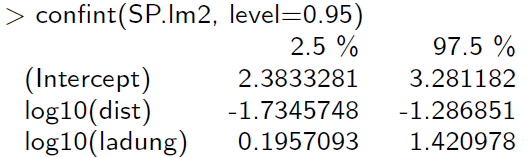
\includegraphics[width=0.3\linewidth]{figures/confint}
	\caption{Beispiel für Konfidenzintervall hier 95\%, \textit{Quelle:} \cite{C:confint}}
	\label{fig:confint}
\end{figure}

\subsubsection{Robuster Schätzer (MM-Schätzer) roblm}
\label{subsubsec:RobSchaetzer}
\begin{figure}[!h]
	\centering
	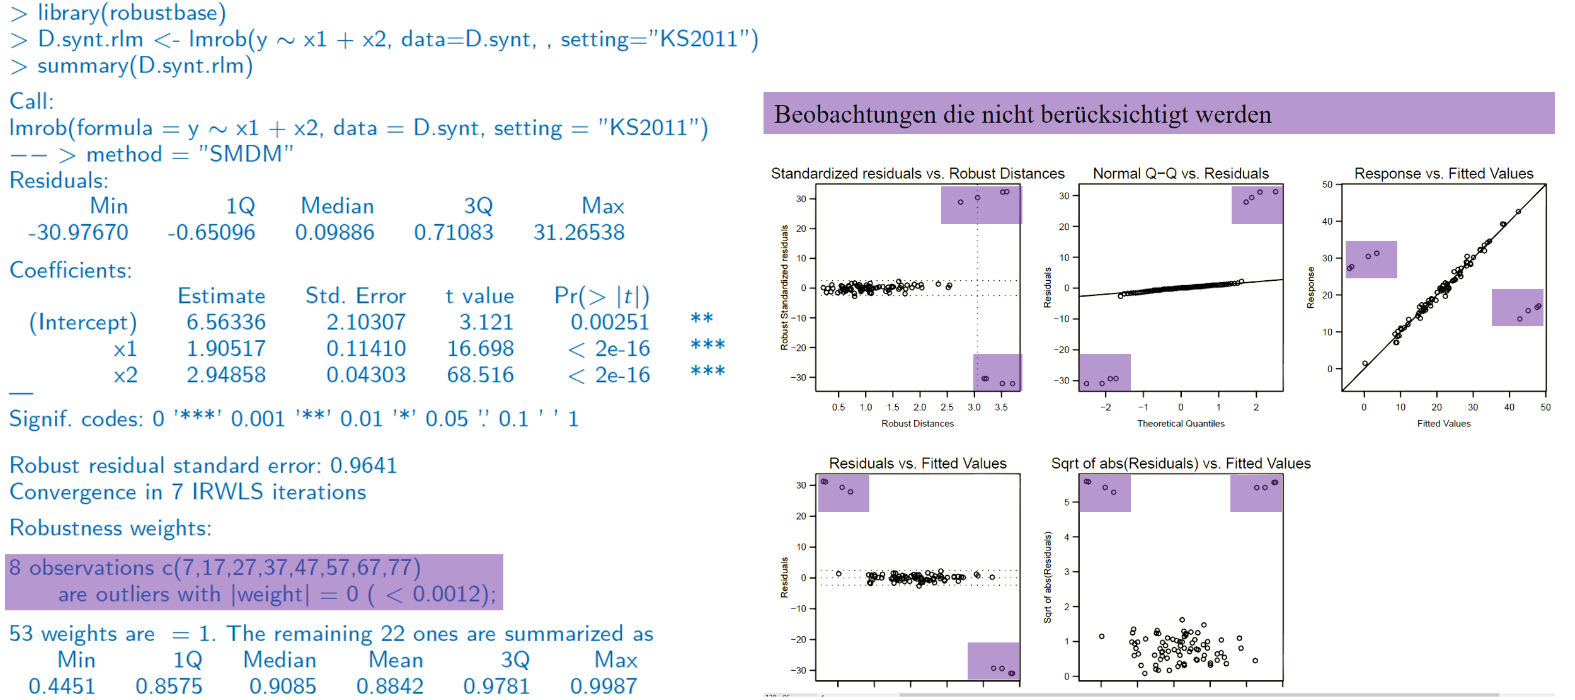
\includegraphics[width=1\linewidth]{figures/roblm}
	\caption{Output des Robusten Schätzers inkl. Zusammenhang mit den verschiedene Plots (Folie 30) \textit{Quelle:}\cite{C:Roblm}}
	\label{fig:roblm}
\end{figure}

\clearpage
\subsubsection{VIF}
\label{subsubsec:VIF}
\begin{figure}[!h]
	\centering
	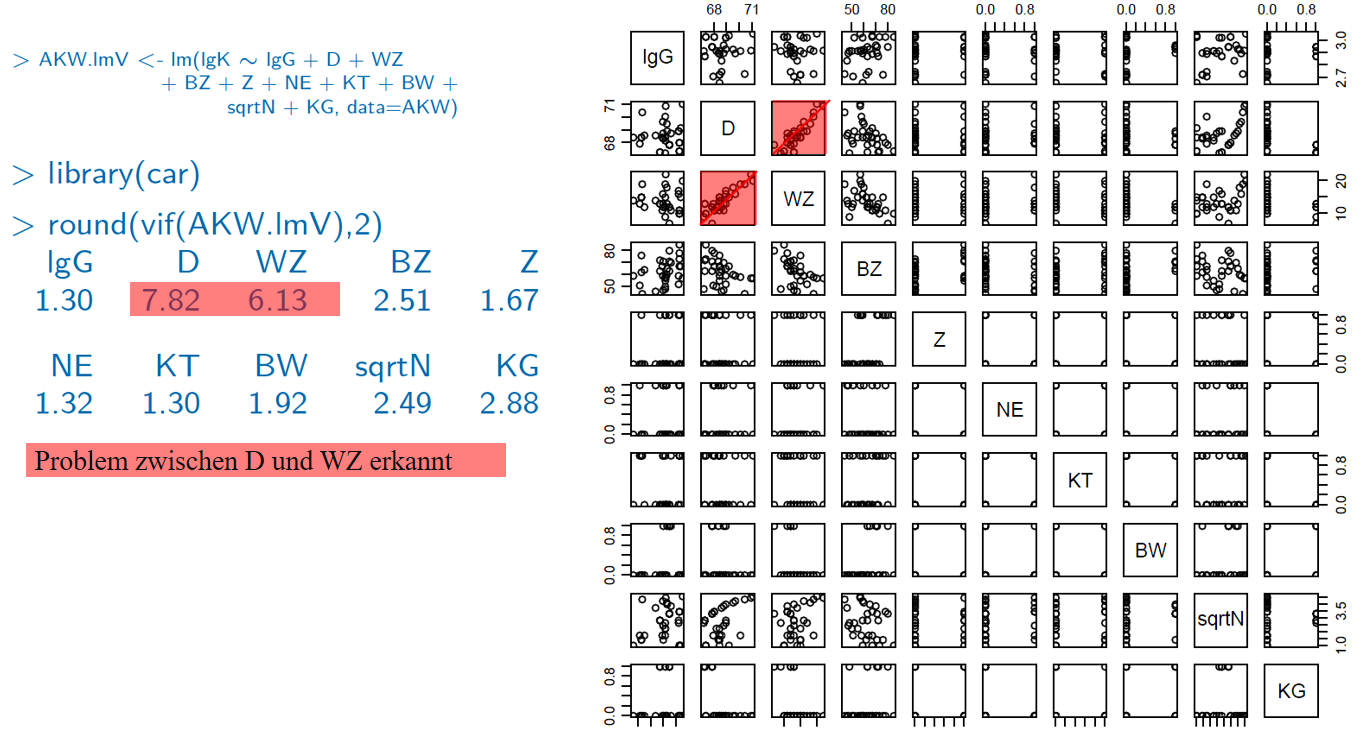
\includegraphics[width=0.9\linewidth]{figures/VIF}
	\caption{Korrelation zwischen zwei Variablen. Zu erkennen an grossem VIF-Wert und ca. linearem Verhalten wenn diese gegeneinader aufgetragen werden \textit{Quelle:} \cite{C:VIF}}
	\label{fig:vif}
\end{figure}

\subsubsection{AIC}
\label{subsubsec:AIC}
\begin{figure}[!h]
	\centering
	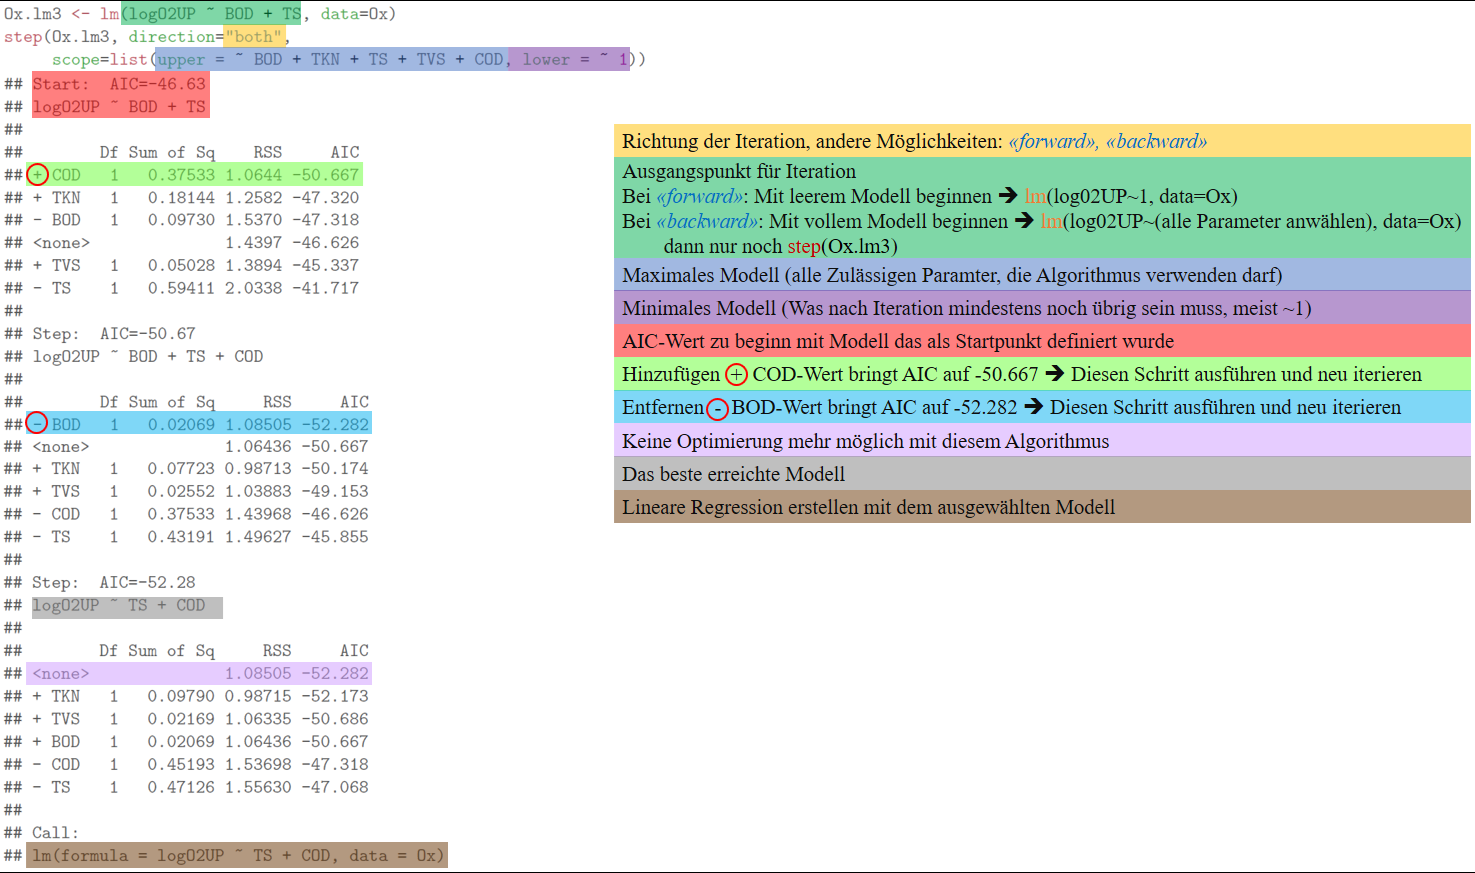
\includegraphics[width=1\linewidth]{figures/AIC}
	\caption{Output von R! für Optimierung nach AIC mit schrittweiser Selektion  \textit{Quelle:} \cite{C:AIC}}
	\label{fig:aic}
\end{figure}
\clearpage

\subsubsection{Dataframe}
\label{subsubsec:Dataframe}
\begin{figure}[h!]
	\centering
	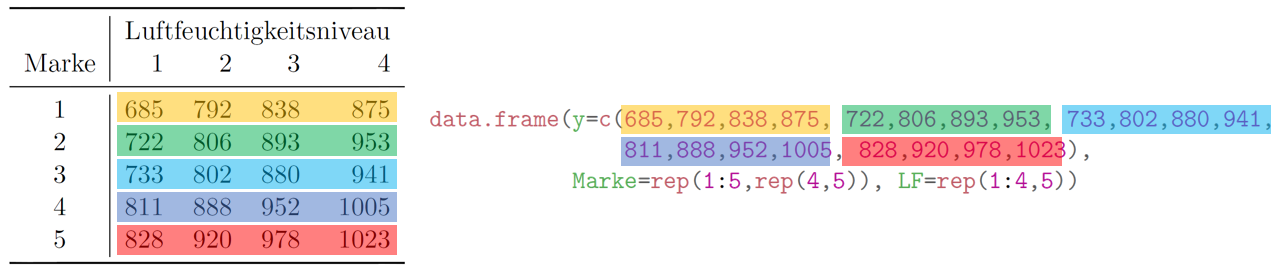
\includegraphics[width=0.7\linewidth]{figures/Dataframe}
	\caption{Manuelle Eingabe von Daten in R! \textit{Quelle:}\cite{C:dataframe}}
	\label{fig:dataframe}
\end{figure}
